\documentclass[runningheads, extrasrussian]{llncs}

%%% Преамбула %%%

\usepackage[T2A]{fontenc}   % кодировка
\usepackage[utf8]{inputenc} % кодировка исходного текста
\usepackage[russian]{babel} % локализация и переносы

\begin{document}

\title{Улучшение алгоритма нахождения Deadlock в Google Thread Sanitizer}

\author{Константин Мазунин \and Олег Доронин \and Андрей Дергачёв}

\authorrunning{Улучшение алгоритма нахождения Deadlock в Google Thread Sanitizer}

\institute{Санкт-Петербургский государственный университет информационных технологий, механики и оптики \and \email{mazuninky@gmail.com}}

\maketitle

\begin{abstract}
Данная работа посвящена исследованию алгоритмов нахождения deadlock в многопоточных приложения, а так же реализации улучшенного алгоритма Google Thread Sanitizer

\keywords{Google Thread Sanitize \and Multithreading \and Deadlock \and Multithreaded errors \and Testing.}
\end{abstract}

\section{Введение}
Взаимоблокировка или Deadlock \cite{ref_pthread} — это ситуация в многозадачной среде, при которой несколько процессов или потоков находятся в состоянии ожидания ресурсов, занятых друг другом, при этом ни один из них не может продолжать свое выполнение. Данная проблема встречается часто в многопоточных приложения и может не только снижать производительность но и приводить к полному “зависанию” всей системы в целом.

\section{Существующие решения}
Возможности нахождения потенциальных Deadlock существуют в таких инструментах, как Google thread sanitizer (GTSAN) \cite{ref_gtsan_github} и Valgrind  \cite{ref_valgrind}. Алгоритм GTSAN базируется на построение графа занятия ресурсов потоками. 

\begin{figure}[htbp]
    \centering
    \begin{subfigure}[h]{0.4\textwidth}
        \centering
        \lstinputlisting[language=C]{inc/2m2t-dd.c}
    \end{subfigure}
    \hfill
    \begin{subfigure}[h]{0.4\textwidth}
        \centering
        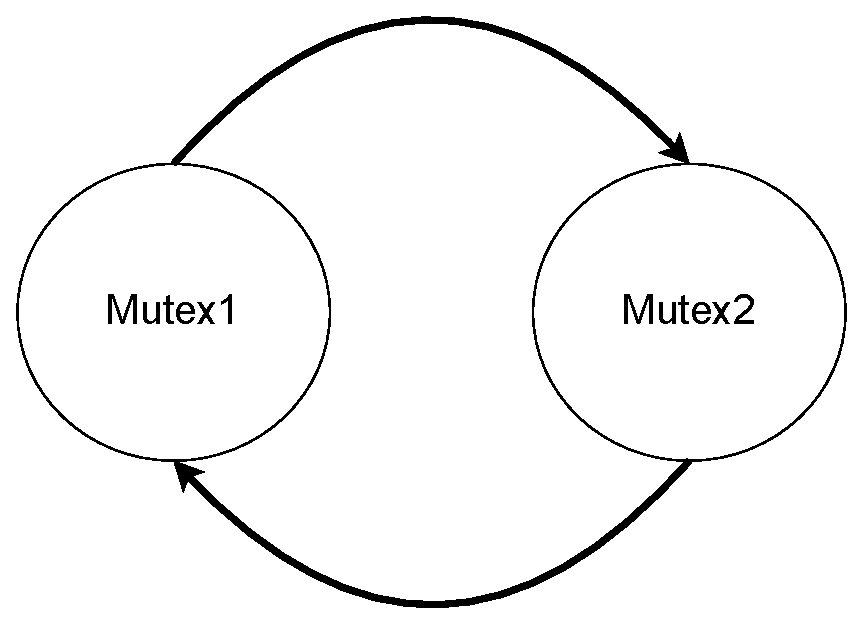
\includegraphics[width=\textwidth]{2m1t.eps}
    \end{subfigure}
    \caption{Фрагмент с взаимоблокировкой на двух потоках}%
    \label{fig:2m2t-d}
\end{figure}

В процессе исполнения программы строится граф, вершинами которого являются мьютексы. В ходе исполнения потока строятся рёбра между последовательным захватом двух мьютексов. После построения графа производится поиск циклов, наличие которых говорит о deadlock. Однако алгоритм имеет ошибки первого и второго рода - ложное срабатывание и пропуск цели.

На Рис. \ref{fig:1m1t-d} происходит ошибка первого рода - ложное срабатывание. Поток, который первым захватит mu1, сможет без взаимной блокировки выполнить захват и освобождение остальных мьютексов, пока второй будет ожидать освобождения mu1. В цикле присуствует граф хотя взаимной блокировки не происходит.

\begin{figure}[htbp]
    \centering
    \begin{subfigure}[h]{0.4\textwidth}
        \centering
        \lstinputlisting[language=C]{inc/3m2t-du.c}
    \end{subfigure}
    \hfill
    \begin{subfigure}[h]{0.4\textwidth}
        \centering
        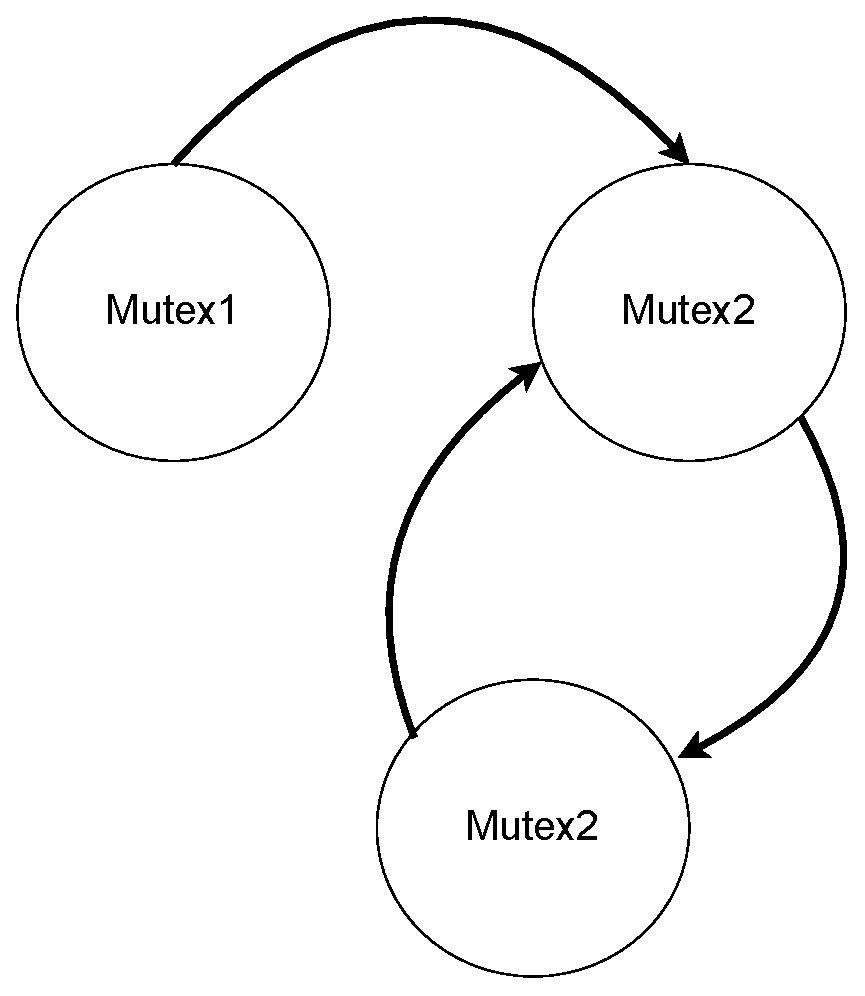
\includegraphics[width=\textwidth]{3m2t-du.eps}
    \end{subfigure}
    \caption{Фрагмент программы с ложной взаимной блокировкой на трёх мьютексах}%
    \label{fig:3m2t-du}
\end{figure}

Рассмотрим примеры с ошибкой второго рода - пропуск цели. На рис \ref{fig:2m2t-du} изображён один из возможных графов поиска взаимной блокировки. Код, который может вызвать взаимную блокировку, исполняется по случайному условию. В зависимости от значения функции rand() программа попадёт в ситуацию взаимной блокировки. Данный алгоритм не может обнаружить случаи, которые происходят в возможных ветвлениях программы.

\begin{figure}[htbp]
    \centering
    \begin{subfigure}[h]{0.4\textwidth}
        \centering
        \lstinputlisting[language=C]{inc/2m2t-du.c}
    \end{subfigure}
    \hfill
    \begin{subfigure}[h]{0.4\textwidth}
        \centering
        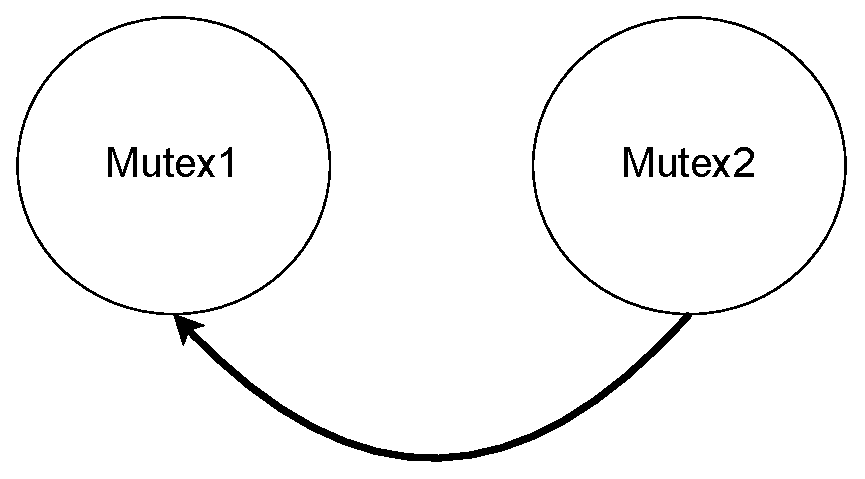
\includegraphics[width=\textwidth]{2m2t-du.eps}
    \end{subfigure}
    \caption{Фрагмент программы с возможным пропуском возможной взаимной блокировки}%
    \label{fig:2m2t-du}
\end{figure}

На Рис. \ref{fig:1m1t-d} происходит блокировка на одном потоке, что не обнаруживает Google thread sanitizer.

\begin{figure}[htbp]
\lstinputlisting[language=C]{inc/1m1t.c}
 \caption{Фрагмент с взаимоблокировкой на одном потоке}%
 \label{fig:1m1t-d}
\end{figure}

При этом Google TSAN и Valgrind не способны обнаружить Deadlock, который произошел уже во время исполнения программы, поэтому в случае возникновения блокировки может быть неясно - это программа долго выполняется или произошёл Deadlock.

\subsection{PostgreSQL} 
В PostgreSQL реализован алгоритм автоматического обнаружения Deadlock\cite{ref_postgre_deadlock}. Рассмотрим пример выполнения двух процессов, приведенный на Рис.~\ref{fig:postgre-flow}.

\begin{figure}[h]
process A: BEGIN;

process B: BEGIN;

process A: UPDATE users SET name = "Peter" WHERE id = 1;

process B: UPDATE users SET name = "Marko" WHERE id = 2;

process A: UPDATE users SET name = "John" WHERE id = 2;

process B: UPDATE users SET name = "John" WHERE id = 1;
\caption{PostgreSQL flow} 
\label{fig:postgre-flow}
\end{figure}

В данном случае процесс A блокирует запись с идентификатором id = 1, а процесс B блокирует запись с идентификатором id = 2. После чего процесс B пытается изменить запись, которую заблокировал процесс A c id = 1, и ждёт пока процесс A завершиться. Аналогичная ситуация происходит и с процессом A, после чего процессы находятся во взаимной блокировке.

PostgreSQL распознает ситуацию, когда два процесса блокируют другу друга, ожидает в течении некоторого интервала времени, после чего выводит ошибку.

\section{Цель работы}

Целью данной работы является улучшение алгоритма обнаружения deadlock, используемого в Google thread sanitizer, дополнением его возможностью обнаружения взаимоблокировок в процессе выполнения программного кода, подобно алгоритму PostgreSQL. Для достижения данной цели предполагается: 
\begin{enumerate}
\item Исследовать существующие реализации алгоритмов обнаружения Deadlock в многопоточных программах;
\item Создать концепцию алгоритма обнаружения Deadlock в режиме исполнения программы.
\end{enumerate}

\section{Реализация}

GTSAN \cite{ref_clang} является инструментом компилятора. Он поставляется вместе GCC и Clang. Механизм работы GTSAN состоит в том, что в ходе компиляции перед операциями с памятью вставляется вызов функции библиотеки GTSAN. В ходе реализации алгоритма было решено использовать данный подход для обнаружения взаимоблокировок в процессе выполнения программного кода. 

\subsection{Алгоритм детектирования}

В ходе исследования был разработан алгоритма, который базируется на построение графа, пример которого приведен на Рис. \ref{fig:my_alg-2m2t} для двух потоков.

\begin{figure}[h]
    \centering
    \begin{subfigure}[h]{0.4\textwidth}
        \centering
        \lstinputlisting[language=C]{inc/2m2t-dd.c}
    \end{subfigure}
    \hfill
    \begin{subfigure}[h]{0.4\textwidth}
        \centering
        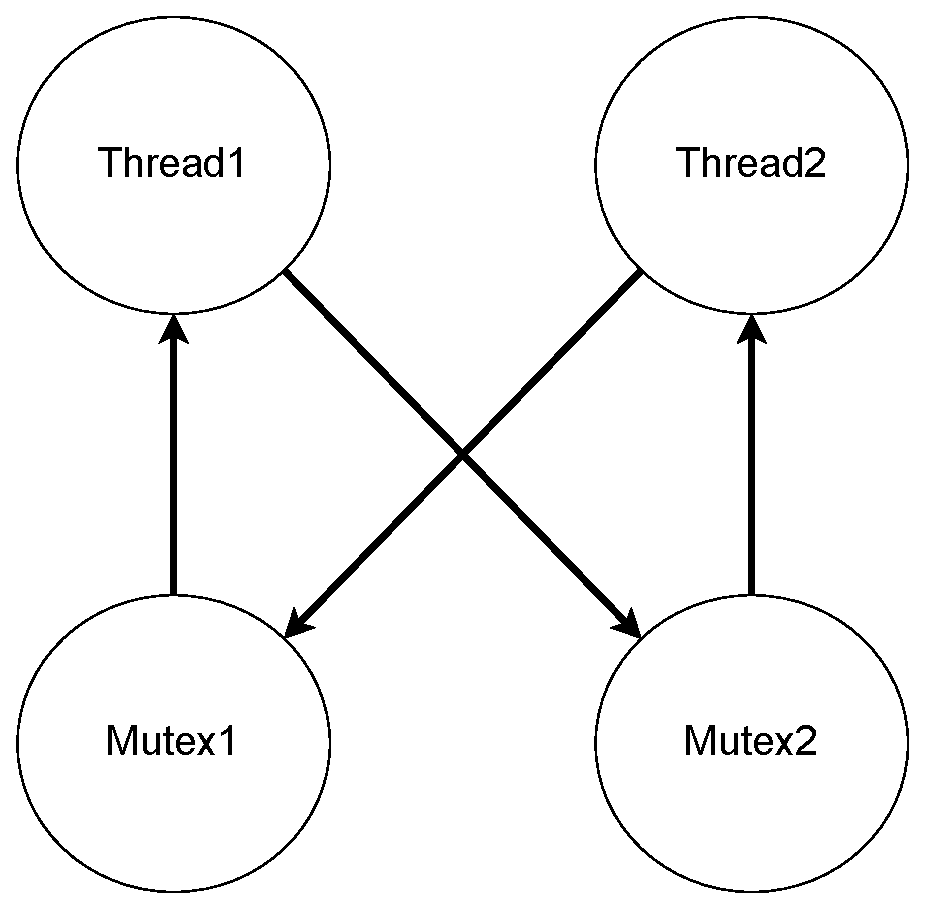
\includegraphics[width=\textwidth]{my_alg-2m2t.eps}
    \end{subfigure}
    \caption{Фрагмент программы с графом детектирования deadlock}%
    \label{fig:my_alg-2m2t}
\end{figure}

Разработанный алгоритм учитывает, в каком потоке захвачен мьютекс, а также какие еще потоки пытаются захватить этот же мьютекс. История захвата мьютекса представлена на Рис \ref{fig:mutex-algo}.

\begin{figure}[h]
T1: mu1, mu2

T2: mu2, mu1
\caption{История захвата мьютекса в потоках} 
\label{fig:mutex-algo}
\end{figure}

На Рис. \ref{fig:mutex-algo} перед двоеточием указано имя потока, а после двоеточия - история захвата мьютексов потоком. Вершинами графа являются потоки и мьютексы. Захваченный потоком мьютекс отображается на графе как направленное ребро от вершины мьютекса к вершине потока. Попытка захвата мьютекса потоком отображается как ребро из вершины потока к вершине мьютекса. Обнаружение цикла в данном графе (как в нашем случае) и будет считаться ситуацией взаимной блокировки, о чем необходимо сообщить пользователю. Из остающихся недостатков данного алгоритма можно отметить, что данный подход применим пока лишь только для обычного mutex.

\subsection{Алгоритм построения графа}

В ходе работы программы необходимо отслеживать действия:
\begin{itemize}
  \item Попытку захвата мьютекса
  \item Захват мьютекса
  \item Освобождение мьютекса
\end{itemize}

Для этих событий необходимо знать поток, который осуществляет это действие, и мьютекс, над которым происходит действие.

Алгоритму необходимо хранить список захваченных мьютексов для каждого потока captured[T,mutlist], где T - поток, а mutlist - список захваченных мьютекс в потоке T, а так же хранить для каждого потока попытку захвата мьютекса try[T, M], где T - поток, а M - захваченный мьютекс.

Далее предстален алгоритм для обработки каждого из действий:

\subsubsection{Попытка захвата мьютекса}
\begin{algorithmic}
\Function{TryMutexLock}{thread, mutex}
    \State $try[thread] = mutex$
\EndFunction
\end{algorithmic}

\subsubsection{Захват мьютекса}
\begin{algorithmic}
\Function{MutexLock}{thread, mutex}
    \State $try[thread] = null$
    \If {$thread \notin captured$}
        \State $captured[thread] = []$
    \EndIf
    \State $captured[thread] = captured[thread] \cup mutex$
\EndFunction
\end{algorithmic}

\subsubsection{Освобождение мьютекса}
\begin{algorithmic}
\Function{MutexFree}{thread, mutex}
    \State $captured[thread] = captured[thread] \textbackslash mutex$
    \If {$captured[thread] = \{\}$}
        \State $captured = captured \textbackslash thread$
    \EndIf
\EndFunction
\end{algorithmic}

Матрица смежности для графа строиться на основе потоков и мьютексов, которые содержаться в captured и try. Для дальнейшего использования использования DFS вершины нумеруются начиная от потоков и заканчивая мьютексами. 

\subsection{Алгоритм поиска пути в графе}

Условием взаимной блокировки в программе является наличие пути в графе. Для алгоритма поиска пути в графе предъявляется условия:
\begin{enumerate}
    \item Минимальна возможная асимптотика
    \item Возможность получить путь, который образует цикл в графе, для дальнейшей интрепритации программой
\end{enumerate}

Для реализации был выбран алгоритм DFS\cite{ref_dsa}, так как он удолетворял условию возможного получения пути для получения цикла, так же его асимптотик для графа  G = (V,E), где V — множество вершин графа, E — множество ребер граф, равняется O(|V|+|E|).

\subsection{Оптимальный алгоритм поиска пути}

В ходе работы программы приходиться перестраивать граф и производить поиск после каждого из событий: попытка захвата мьютекса, захват мьютекса, освобождение мьютекса. Чтобы не приходилось каждый раз производить поиск цикла в графе, необходимо использовать структуру, которая позволяет хранить предыдущий результат поиска циклов в графе и обновляеть её при каждой операции добавления или удаления вершины из графа.

Данная проблема была решена в работе "Real-time Constrained Cycle Detection in Large DynamicGraphs" \cite{ref_dynamic_cycle}, в которой представлен алгоритм поиска цикла в динамических графах, что позволяет за меньшее время находить цикл в графе, но увеличивает потребление памяти программой.

\subsection{Интерпретация цикла в графе}

Для конечного пользователя необходимо интепретировать путь в графе как ресурсы из-за которых произошла взаимная блокировка, то есть вывести данных о потоках и мьютекса, которые привели к данной ситуации.

Рассмотрим ситуацию с Рис. \ref{fig:my_alg-2m2t}. Для алгоритма DFS пронумеруем сначала потоки, а потом мьюксы. Соотвественно Thread1 - вершина номер 1, Thread2 - вершина номер 2, Mutex 1 - вершина номер 3,  Mutex 2 - вершина номер 4. Алгоритм поиск цикла вернёт вершины в таком порядке: [1, 4, 2, 3]. Пронумеруем элементы списка вершин в цикле от 1 до 4, то есть элементом номер 1 будет 1 вершина, а элементом под номером 4 будет 3 вершина.

Результат работы алгоритма можно интерпретировать как: элемент 1 захватил элемент 3 и пытается захватить элемент 2, пока элемент 3 захватил элемент 4 и пытается захватить элемент 3.

\section{Заключение}

В ходе данной работы были рассмотрены существующие алгоритмы обнаружения Deadlock, а также предложена и реализована концепция улучшенного алгоритма Google Thread Sanitizer, которая использует принцип, похожий на метод обнаружения deadlock в PostgreSQL.

\begin{thebibliography}{8}
\bibitem{ref_pthread}
Bil LewisDaniel, J. Berg. PThreads Primer - 2th Edition. BergSunSoft Press, 1996, p. 42

\bibitem{ref_gtsan_github}
Github, \url{https://github.com/google/sanitizers/wiki/ThreadSanitizerDeadlockDetector}.  Last accessed 10 Nov 2019

\bibitem{ref_valgrind}
Valgrind, \url{http://valgrind.org/docs/manual/hg-manual.html}. Last accessed 10 Nov 2019

\bibitem{ref_postgre_deadlock}
Shiroyasha, \url{http://shiroyasha.io/deadlocks-in-postgresql.html}. Last accessed 10 Nov 2019 

\bibitem{ref_clang}
LLVM, \url{https://clang.llvm.org/docs/ThreadSanitizer.html}. Last accessed 10 Nov 2019 

\bibitem{ref_dsa}
Lecture Notes forData Structures and Algorithms,\url{https://www.cs.bham.ac.uk/~jxb/DSA/dsa.pdf}. Last accessed 10 Nov 2019

\bibitem{ref_dynamic_cycle}
Xiafei Qiu, Wubin Cen, Zhengping Qian, You Peng, Ying Zhang,Xuemin Lin, and Jingren Zhou.  Real-time Constrained CycleDetection in Large Dynamic Graphs.PVLDB, 11 (12): 1876-1888, 2018.DOI: \url{https://doi.org/10.14778/3229863.3229874}
\end{thebibliography}
\end{document}